%%%%%%%%%%%%%%%%%%%%%%%%%%%%%%%%%%%%%%%%%%%%%%%
% BEGIN NEWTON's WETTEN
%%%%%%%%%%%%%%%%%%%%%%%%%%%%%%%%%%%%%%%%%%%%%%%

\chapter{Newton's wetten}\label{chap:newton}

In dit hoofdstuk komen de drie wetten van Newton aan bod. Deze wetten vormen het hart
van de klassieke mechanica en sommige begrippen zijn houdbaar ook buiten
de klassieke mechanica. De wetten van Newton vormden een revolutie in de
natuurwetenschappen en hebben de basis gelegd voor de exacte - mathematische - beschrijving
van de natuur zoals we die nu kennen.

Naast de wetten van Newton zelf worden in dit hoofdstuk een paar veel in de natuur 
voorkomende krachten behandeld.

Stof uit Giancoli:
\begin{itemize}
\item Hoofdstuk 4
\item Hoofdstuk 5.1 en 5.6
\end{itemize}

\section{Eerste wet {\it of }  "Dat eens roert, roert altijt, soot niet belet wort"}\label{sec:newton1}

De eerste van de drie wetten van Newton is een uitspraak over de relatie tussen krachten en
beweging van een object. 

\begin{Newton1}
Een object waarop de netto kracht gelijk is aan nul, beweegt met een constante snelheid (of is en blijft in rust).
\end{Newton1}

De eerste wet van Newton vertelt ons dus dat als we de snelheid van een object willen 
veranderen, daarvoor een kracht nodig is. Heel simplistisch gezien lijkt het bijna
een betekenisloze uitspraak: je moet iets doen om iets te veranderen. Toen Newton
zijn eerste wet op schrift stelde, was het echter niet minder dan een revolutionaire gedachte
(eerlijk is eerlijk: Galilei had hetzelfde idee ook min of meer gehad, maar dat was dan ook
een behoorlijk slimme kerel). Eeuwenlang had men het gedachtegoed van Aristoteles en zijn 
oude Griekse vrienden gekoesterd en die beweerden het tegenovergestelde: namelijk dat
elk object een 'natuurlijke drang' heeft om tot rust te komen en dat je zelf iets moet doen
om een beweging aan de gang te houden.  Deze kijk op de natuur is natuurlijk niet zo wonderlijk, 
omdat dat strookt met onze dagelijkse waarnemingen. Als je een willekeurig object een zetje geeft 
komt ie in beweging en stopt ie na een meestal korte tijd weer. Newton verklaart dit tot stilstand
komen niet met een natuurlijke drang, maar uit het feit dat er {\it dus} een kracht op dit object werkt.
({\it vraag: een schaatser maakt snelheid, glijdt een eindje en komt tot stilstand. Verklaar zowel 
aan de had van de oude Grieken en aan de hand van Newton en Galilei.})

Het is van belang te onderzoeken wanneer Newtons eerste wet geldt. Wanneer je in 
een trein zit die versnelt en er ligt een bal op de vloer, dan versnelt die bal , zonder dat er 
een kracht op die bal lijkt te werken. In versnelde systemen werkt Newton's eerste wet 
blijkbaar niet ({\it vraag: is dat vreemd?}). In het algemeen geldt Newton's eerste wet in systemen 
die met een constante snelheid ten opzichte van elkaar bewegen: ook 'stilstaande' systemen
zijn hiervoor dus prima geschikt. Vaak nemen we een stilstaand coordinatensysteem
dat we definieren ten opzichte van een vast punt op het oppervlak van de aarde als 
referentiesysteem, hoewel dat niet helemaal correct is ({\it waarom niet?}). Dergelijke systemen,
waarin de eerste wet van Newton geldt noemen we {\bf inertiaalstelsels}. 

\section{Tweede wet}

De eerste wet van Newton legt een relatie tussen kracht en snelheidverandering. Newton's
tweede wet legt vast hoe die relatie precies in elkaar zit.
\begin{Newton2}
De versnelling van een object is evenredig met de netto kracht die op het object wordt
uitgeoefend:
\begin{equation}\label{eq:newton2}
\vec{F}_{tot} = \sum \vec{F} = m \vec{a}
\end{equation}
\end{Newton2}
De evenredigheidsconstante tussen de kracht en de versnelling is wat wij kennen
als de massa, $m$, van dat object.  Een grote massa is moeilijker in beweging te krijgen
dan een kleine massa. Een grote kracht leidt tot een grote versnelling. Precies zoals we 
verwachten dus.  De meesten van jullie kunnen we op een willekeurig moment wel 
wakker maken voor opdreunen van deze formule, maar toch is dit niet de meest gebruikelijke
notatie voor het schrijven van Newton's tweede wet. Als we het begrip impuls, 
$\vec{p}=m\vec{v}$ uit het vorige hoofdstuk er weer bij halen, en de afgeleide nemen naar
de tijd, zie je dat we vgl.~\ref{eq:newton2} ook kunnen schrijven als:
\begin{equation}
\vec{F}_{tot} = \frac{d \vec{p}}{dt}
\end{equation}
In deze vorm wordt de tweede wet van Newton het liefst gebruikt: een kracht leidt tot
een verandering van impuls. Deze relatie tussen impuls en kracht maakt impuls zo'n enorm
belangrijke grootheid binnen de klassieke mechanica en daarbuiten. De tweede wet van Newton
is perfect consistent met  de eerste wet - eigenlijk is het een meer wiskundige manier van hetzelfde
statement. Wanneer de kracht in vgl.~\ref{eq:newton2} gelijk aan nul is, is de versnelling
nul, en de snelheid dus constant. Net zoals de eerste wet je vertelt.

\begin{center}
\line(1,0){250}
\end{center}

\begin{voorbeeld} 
\label{ex:newton:kracht}
 \begin{figure}[htbp]
\begin{center}
  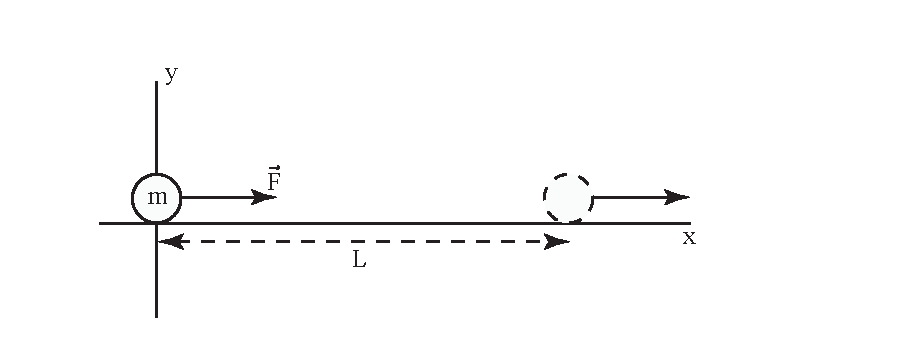
\epsfig{file=Versnelling.pdf, width=\textwidth}
\caption{{\it Kracht en versnelling.}}
\label{fig:newton:wet2}
\end{center}
\end{figure} 
Je trekt met een kracht $\vec{F}$ aan een object met massa $m$. Van wrijving of andere
soorten weerstand is geen sprake. Hoe lang doe je er over om een afstand $L$ af te leggen als
het object op $t=0$ in rust is?

{\bf Oplossing: }{\it Laten we ervoor kiezen om de kracht op ons object te laten werken in de $x$ richting,
 zoals aangegeven in Fig.~\ref{fig:newton:wet2}: er geldt dan $\vec{F} = (F, \, 0,\,0)$. 
 De versnelling wordt
 dan gegeven door $\vec{a}=(F/m, \,0,\,0)$. Als we nu de vergelijking voor eenparig versnelde beweging
 weer uit de kast halen krijgen we:
 \begin{equation}
 \vec{r}(t) = \left(\begin{array}{c}
  x(t) \\
  y(t) \\
  z(t) 
  \end{array}\right)
  = \frac{1}{2}\left(\begin{array}{c}
  (F/m) \, t^2 \\
  0 \\
  0
 \end{array}\right)
  + \vec{0} \, t + \vec{0}
 \end{equation}
 De laatste twee vectoren geven aan dat de initiele snelheid nul is, $\vec{v}_0 = \vec{0}$ en dat de initiele
 positie van het object in de oorsprong ligt $\vec{r}_0 = \vec{0}$. Deze laatste heb ik zo gekozen uit gemak.
 Oplossen voor $x(t)=L$ geeft:
 \begin{equation}
 t = \sqrt{\frac{2 \,m \,L}{F}}
 \end{equation}
 Vraag: check of de dimensies kloppen.
 }
\end{voorbeeld}

\begin{center}
\line(1,0){250}
\end{center}


\section{Derde wet}

De derde wet van Newton behandelt de vraag hoe nou precies krachten worden uitgeoefend
tussen objecten. Newton heeft dit mechanisme samengevat in zijn bekende actie is reactie wet:
\begin{Newton3}
Als een object een kracht uitoefent op een tweede object, dan oefent dat tweede object een
evengrote kracht uit op het eerste object in tegengestelde richting.
\end{Newton3}
of:
\begin{equation}
\vec{F}_{1\rightarrow2} = - \vec{F}_{2\rightarrow1}
\end{equation}
Op het eerste gezicht lijkt deze wet triviaal, want als ik bijvoorbeeld stil op de grond sta, dan
trekt de zwaartekracht mij naar beneden, terwijl de grond even hard naar boven duwt. De 
totale kracht op mij is gelijk nul, en ik blijf dus onversneld (=stil) staan. Maar Newton postuleerde
dat ook als een object wel versneld wordt, de kracht die zorgt voor de versnelling een even
grote reactie-kracht opwekt.

Je zou jezelf nu de vraag kunnen stellen hoe het mogelijk is dat er uberhaupt iets in 
beweging gezet kan worden, aangezien de som der krachten altijd nul is. Voor iedere
kracht is er immers een reactiekracht van tegengesteld teken. Het antwoord op die vraag
ligt in het feit dat je je altijd moet afvragen {\it waarop} een bepaalde kracht wordt uitgeoefend.
Als ik bijvoorbeeld een krijtje het publiek in wil gooien tijdens een college, dan oefen ik
daarvoor een kracht uit op het krijtje. De reactiekracht volgens Newton's derde wet is tegengesteld
aan deze kracht, maar deze wordt uitgeoefend op mijn hand en niet op het krijtje. Op
het krijtje wordt dan wel degelijk een netto kracht uitgeoefend en daardoor wordt deze 
versneld.

Het voorbeeld hierboven van het krijtje wordt trouwens op grote schaal gebruikt bij
voortstuwing van bijvoorbeeld raketten. Een raket stoot
enorme hoeveelheden gassen met een hoge snelheid uit de motor. Bij deze
uitstoot worden de gassen enorm versneld en de raket oefent dus een grote kracht
uit op deze gassen. Volgens Newton's derde wet is er een reactiekracht even groot in 
tegengestelde richting die wordt uitgeoefend op de raket door deze gassen. Het is precies
deze reactiekracht die ervoor zorgt dat een raket zich voortbeweegt, en niet zoals je
vaak hoort door het afzetten van de gassen tegen de grond of de omliggende lucht. Stel dat een
raket zich wel zou afzetten tegen de atmosfeer of de grond. Hoe zou zo'n beest dan moeten
versnellen als ie eenmaal buiten de dampkring is?

\section{Krachten van verschillende soorten}

In deze paragraaf passeren er verschillende typen krachten de revue met als doel dat je het
gereedschap hebt om eenvoudige krachten analyses te doen. Een dergelijke krachten analyse
volgt altijd min of meer hetzelfde patroon. Je begint met een schets te maken van het fysische
probleem, waarmee wordt bedoeld een tekening van alle relevante objecten en krachten die
worden uitgeoefend. Als je hebt geanalyseerd welke krachten van belang zijn, ben je in staat
de netto-kracht en dus versnelling van een object uit te rekenen. Meestal is de wiskunde voor
dergelijke problemen eenvoudig. Wat lastig is, is een goede en trefzekere analyse van het 
probleem om de krachten op je object te bepalen. Uiteraard moet je er bij dergelijke analyses altijd
rekening mee houden dat je te maken hebt met vectoren. In de rest van de paragraaf worden 
meer en meer krachten geintroduceerd en zal je in staat zijn ingewikkelder problemen op
te lossen.

\subsection{Zwaartekracht \& Normaalkracht}

De eerste kracht die aan bod komt zal niet verrassend de zwaartekracht zijn. Bij de problemen
die we in dit hoofdstuk tegenkomen zal de zwaartekracht, $\vec{F}_G$ op een object met massa
$m$  worden gegeven door:
\begin{equation}\label{eq:zwaartekracht}
\vec{F}_G = m \vec{g}
\end{equation}
waarbij $\vec{g}=(0,\,0,\,-9.8m/s^2)$ de zwaartekrachtsversnelling aan het oppervlak van de aarde.
Let hierbij op het min-teken voor de zwaartekrachtsversnelling, aangezien ik de positieve
$z$-as van mijn coordinaten systeem het liefste omhoog laat wijzen.  Let wel goed op dat
vgl.~\ref{eq:zwaartekracht} alleen geldig is aan het oppervlak van de aarde. Wanneer we de ruimte in
gaan dan moeten we Newton's zwaartekrachtwet gebruiken die netjes de zwaartekracht  beschrijft
als functie van de afstand tot een object (bv. de aarde). Ook als we opgaven gaan doen op een 
andere planeet moet je ermee rekening houden dat $\vec{g}$ wel eens anders kan zijn. 
Het is trouwens wel opmerkelijk (dat vond Einstein tenminste) dat de massa die horen bij
de tweede wet van Newton, $\vec{F}=m\vec{a}$ precies dezelfde massa is als die hoort
bij de zwaartkrachtvergelijking~\ref{eq:zwaartekracht}. Het gevolg is dat objecten ongeacht
hun massa precies dezelfde versnelling ondergaan! Deze equivalentie tussen {\it trage} en
{\it zware} massa is tot op grote nauwkeurigheid experimenteel aangetoond en vormt
een van de fundamenten van de algemene relativiteitstheorie van Einstein.

Een vaste partner van de zwaartekracht is de zogenaamde normaalkracht. Als docent Colijn
met zijn volle gewicht op de grond staat werkt de zwaartekracht op hem, terwijl hij toch niet
door de grond zakt. De kracht die terugduwt heet de normaalkracht, meestal weergegeven
door $\vec{F}_N$. 
 \begin{figure}[htbp]
\begin{center}
  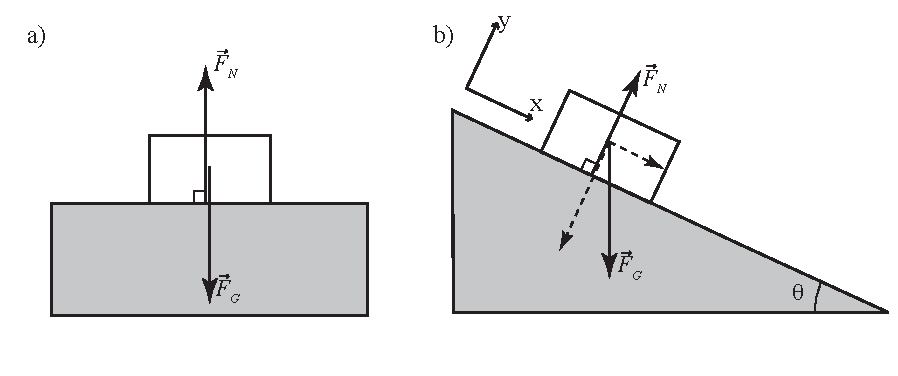
\epsfig{file=NormaalKracht.pdf, width=\textwidth}
\caption{{\it a) Zwaartekracht en normaalkracht voor een horizontaal oppervlak. b) Hetzelfde maar
nu voor een oppervlak dat onder een hoek $\theta$ staat.}}
\label{fig:norm}
\end{center}
\end{figure} 
De normaalkracht staat {\it altijd} loodrecht op het oppervlak dat deze kracht uitoefent,
dus als het oppervlak waarop een object zich bevind horizontaal is, zal de normaalkracht 
precies even groot zijn als de zwaartekracht zoals aangegeven in Fig.~\ref{fig:norm}~a). 
Wat verder belangrijk is om  te zien in Fig.~\ref{fig:norm} is waar de zwaartekracht en de 
normaalkracht aangrijpen. De zwaartekracht wordt altijd getekend vanuit het zwaartepunt of 
massa-middelpunt (wordt later nog behandeld), terwijl de normaalkracht aangrijpt bij het contact
tussen het oppervlak en het object.

Als  het object - Colijn in dit geval - zich op een hellend vlak begeeft wijst de normaalkracht 
nog steeds
loodrecht op het oppervlak, zodanig dat de component van de zwaartekracht in de richting van het 
oppervlak precies wordt opgeheven, zoals in Fig.~\ref{fig:norm}b).  Wat denk je dat er zou 
gebeuren als dit niet het geval zou zijn? Mochten er verder geen wrijving 
of andere krachten in het spel zijn dan zorgt de component van de zwaartekrachtsversnelling 
langs de helling voor de versnelling van de docent. Realiseer je wel dat niet alleen de 
zwaartekracht een normaalkracht kan veroorzaken: ook als je bijvoorbeeld hard tegen een muur 
aanduwt zorgt de normaalkracht, die even grot is als de kracht waarmee je duwt, ervoor dat je 
hand niet door de muur heengaat.

\begin{center}
\line(1,0){250}
\end{center}

\begin{voorbeeld} 
\label{ex:normaalkracht}
Stel dat de massa van het object op de helling in Fig.~\ref{fig:norm} gegeven is door $m$. 
Wat is (i) de normaalkracht op het object (ii) de versnelling? 

{\bf Oplossing: } {\it De normaalkracht is de reactiekracht die de component van de zwaartekracht 
loodrecht op het oppervlak compenseert. Het is in dit geval handig om een coordinatensysteem te 
kiezen waarbij de $x$-as parallel aan het schuine oppervlak staat en de $y$-as loodrecht daarop. 
(i) In dit coordinatensysteem geldt voor de normaalkracht:
\begin{equation}
\vec{F}_N = m \, g \left(\begin{array}{c}\
0 \\
\cos\theta
\end{array}\right)
\end{equation} 
De grootte van $\vec{F}_N$ is dus $m\,g\,\cos\theta$. (ii) Voor de grootte van de kracht langs het
oppervlak geldt dan $|\vec{F}_{par}|=m\,g\,\sin\theta$ en voor de versnelling hoeft nog slechts
gedeeld te worden door $m$.
 }
\end{voorbeeld}
\begin{center}
\line(1,0){250}
\end{center}

Een laatste belangrijke opmerking over normaalkrachten: dit zijn de krachten die uiteindelijk
bepalen hoeveel gewicht je aangeeft op een weegschaal. Namelijk door op een weegschaal
te gaan staan (moet wel horizontaal staan) zorgt de zwaartekracht ervoor dat de weegschaal
een normaalkracht op jou moet uitoefenen die gelijk is aan de zwaartekracht. Je meet dus
op een weegschaal dus ook niet je massa (hoewel die wel op het metertje staat aangegeven), 
maar je meet het effect van de zwaartekracht op jouw hoeveelheid massa. Als je de
weegschaal meeneemt naar de maan zal je slechts een fractie van je gewicht meten omdat
$g$ op de maan veel kleiner is. Je massa is natuurlijk hetzelfde gebleven (als je tenminste
niet bent afgevallen van de raketreis). 

\subsection{Spankracht}

Heel kort een veelvoorkomende kracht: de spankracht in een flexibel koord met
vaste lengte en massa $m=0$. Als je met een dergelijk touw aan een object trekt dan
kan je drie dingen direct opmerken over de krachten in het koord. Ten eerste moet
de kracht in het koord - spankracht of $\vec{F}_T$ genoemd - in dezelfde richting
staan als het koord zelf. Zou dit niet het geval zijn dan zorgt het koord er voor dat 
ie toch in de richting van de kracht komt te staan in de kleinst mogelijke tijd. Het
koord is immers flexibel en heeft $m=0$ ({\it probeer dit argument te begrijpen met
redenatie uit ongerijmde~\footnote{Bij een redenatie uit het ongerijmde laat je zien dat het tegendeel van 
je stelling leidt tot een contradictie}}). Ten tweede moet de krachten op beide uiteinden van
het koord hetzelfde zijn met tegengesteld teken.  Tenslotte kan je aan een dergelijk 
flexibel koord alleen maar trekken. Duwen met een draadje is niet mogelijk, maar
dat zal je wel niet verbazen.

\begin{center}
\line(1,0){250}
\end{center}
\begin{voorbeeld} 
\label{ex:spankracht}
Twee massa's $m_B$ en $m_A$ zijn met elkaar verbonden door middel van een touw. Je
trekt met kracht $\vec{F}_P$ aan de twee massa's zoals aangegeven in Fig.~\ref{fig:span}. 
Wat is (i) de versnelling van beide massa's en (ii) de spankracht in het touw als we ervan
uitgaan dat er geen wrijving is?

\begin{figure}[htbp]
\begin{center}
  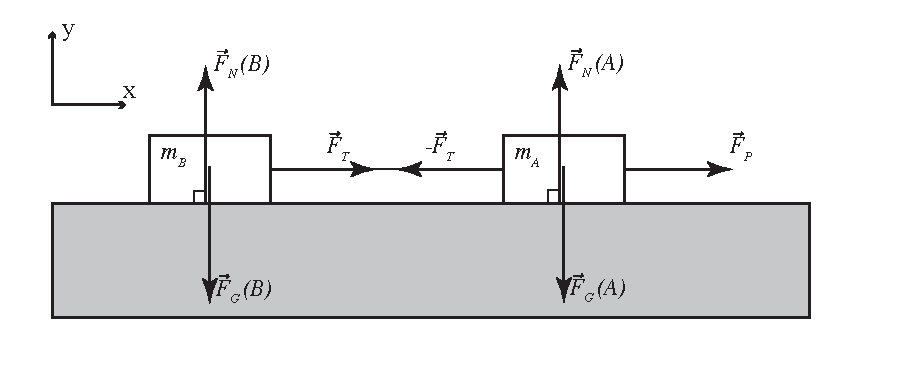
\epsfig{file=SpanKracht.pdf, width=\textwidth}
\caption{{\it Massa A en B worden voortgetrokken en zijn verbonden door middel van een touw.}}
\label{fig:span}
\end{center}
\end{figure} 
{\bf Oplossing: } {\it Begin bij het oplossen van een dergelijk probleem {\it altijd} met het
maken van een tekening van alle relevante krachten. Is ook belangrijk op een tentamen, omdat
er anders geen punten worden gegeven. We kijken eerst naar massa B en zien dat er in totaal
drie krachten op deze massa werken, een spankracht, de zwaartekracht en een normaalkracht.
Dus:
\begin{equation}
\vec{F}_T +\vec{F}_G(B)+\vec{F}_N(B)= m_B\, \vec{a}_B
\end{equation}
Het lijkt misschien een beetje overdreven om hier alle krachten op te schrijven, omdat we toch
niet echt geinteresseerd zijn in beweging in de $y$ richting. In de $y$-richting gebeurt er niet
zoveel zolang de massa's niet loskomen van het oppervlak: de normaalkracht heft precies de
zwaartekracht op. We kunnen ons in dit geval dus
net zo goed beperken tot het opschrijven van alleen de $x$ component van de krachten
en versnelling. Voor massa A en B wordt dit:
\begin{eqnarray}
F_{P\,x} - F_{T\,x} & = & m_A\,a_{A\,x}\\
F_{T\,x} & = & m_B\,a_{B\,x} 
\end{eqnarray}
Beide versnellingen moeten wel aan elkaar gelijk zijn $\vec{a}=\vec{a}_A=\vec{a}_B$, omdat het touw niet kan uitrekken. We
hebben dan twee vergelijkingen met twee onbekenden waaruit we (i) vinden
\begin{equation}
|\vec{a}| = \frac{|\vec{F}_P|}{m_A+m_B}
\end{equation}
en (ii) voor de spankracht:
\begin{equation}
|\vec{F}_T| = \frac{m_B}{m_A+m_B}\,|\vec{F}_P|
\end{equation}

 }
\end{voorbeeld}
\begin{center}
\line(1,0){250}
\end{center}

\subsection{Wrijving}\label{sec:wrijving}

Tot nu toe hebben we aangenomen dat alle beweging gebeurt zonder wrijving. Dit is
uiteraard een onhoudbare simplificatie van de meeste natuurkundige problemen in 
de klassieke mechanica, en zonder wrijving stroken de meeste berekeningen dan ook niet
met onze dagelijkse ervaringen. In deze paragraaf komt wrijving aan bod tussen twee
oppervlakken die met elkaar contact maken. We moeten bij wrijving een duidelijk
onderscheid maken tussen twee vormen van wrijving: {\it kinetische} en {\it statische}. 

Kinetische wrijving is de wrijvingskracht die een object ondervindt wanneer deze
langs een oppervlak beweegt. De wrijvingskracht, $\vec{F}_{fr}$~\footnote{Het subscript
$fr$ komt van het Engelse woord voor wrijving, friction. Deze notatie wordt gebruikt in
Giancoli.} is tegengesteld aan de richting van de beweging en de grootte is evenredig 
met de normaalkracht:
\begin{equation}
|\vec{F}_{fr}| = \mu_{k} |\vec{F}_N|
\end{equation}
De evenredigheidsconstante $\mu_k$ heet de coefficient van kinetische wrijving, en deze
moet empirisch worden bepaald. Een microscopisch model voor het uitrekenen van 
wrijvingskrachten is praktisch niet te realiseren, omdat je voor het uitrekenen van $\mu_k$ 
gecompliceerde grootheden als moleculaire aantrekkingskrachten, ruwheid van oppervlakten 
en dergelijke nodig hebt. Experimentele waarden voor $\mu_k$ liggen tussen 0.01 ({\it
wat zou de eenheid van $\mu$ zijn}) voor goed geoliede kogellagers tot 0.4 voor
bijvoorbeeld het bewegen van hout op hout.

Naast kinetische wrijving heb je uiteraard ook te maken met wrijving als je tegen een
object dat nog niet in beweging is: dit heet statische wrijving. Zolang een object niet
beweegt is de wrijvingskracht even groot als de kracht die werkt langs het oppervlak wordt
uitgeoefend. De maximale wrijvingskracht waarbij een object nog net niet in beweging komt
wordt gegeven door:
\begin{equation}\label{eq:wrijvingstatisch}
|\vec{F}_{fr}| = \mu_s |\vec{F}_N|
\end{equation}
Wederom is de kracht evenredig met de normaalkracht die het object uitoefent, maar
nu met de coefficient van statische wrijving, $\mu_s$. Dus denk 
er om dat de wrijvingskracht zolang een object stilstaat even groot is als de kracht die
wordt uitgeoefend langs het oppervlak. Vgl.~\ref{eq:wrijvingstatisch} geeft het \emph{maximum}
aan van deze kracht. In het algemeen geldt:
\begin{equation}\label{eq:wrijvingscoef}
\mu_s \geq \mu_k
\end{equation}
De statische wrijvingskracht is groter dan de kinetische. Dit strookt met dagelijkse ervaringen
als je bijvoorbeeld denkt aan het verschuiven van een zware doos op een parketvloer. Als
de doos eenmaal in beweging is kost het minder moeite om de doos in beweging te houden. 
Stel nou eens dat $\mu_s<\mu_k$. In dat geval zou de wrijvingskracht tijdens bewegen 
groter moeten zijn dan tijdens stilstand: het zal je dan niet lukken een object van z'n plek
te krijgen! Dus het moet wel zo zijn dat vgl.~\ref{eq:wrijvingscoef} geldt.

\begin{center}
\line(1,0){250}
\end{center}
\begin{voorbeeld} 
\label{ex:wrijving1}
Je trekt aan een object met massa $m$ net zo hard dat ie net in beweging komt, zoals
in Fig.~\ref{fig:wrijving1}~a). Wat is de versnelling als de coefficienten van statische en
kinetische wrijving respectievelijk $\mu_s$ en $\mu_k$ heten?
\begin{figure}[htbp]
\begin{center}
  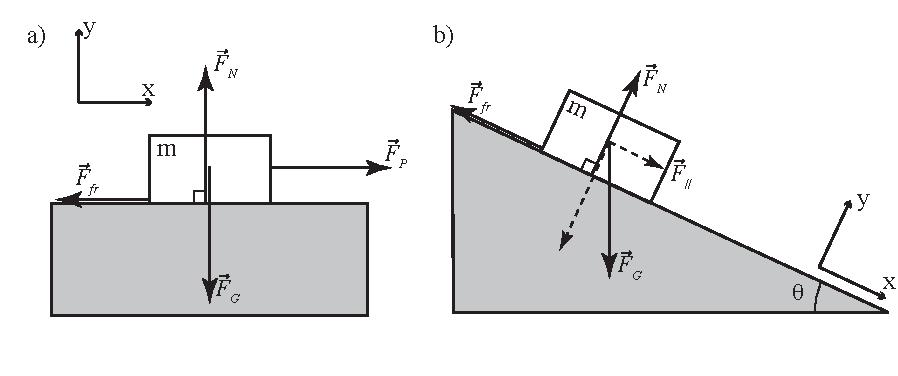
\epsfig{file=Wrijvingskracht.pdf, width=\textwidth}
\caption{{\it a) Wrijvingskracht in het horizontale vlak en b) op een hellend vlak.}}
\label{fig:wrijving1}
\end{center}
\end{figure} 

{\bf Oplossing: } {\it  Om het object te laten bewegen moet je trekken met een kracht
die tenminste net zo groot is als de maximale wrijvingskracht. Dus:
\begin{equation}
\vec{F}_P = (\mu_s |\vec{F}_N|,\,0,\,0) = (\mu_s\,m\,g,\,0,\,0)
\end{equation}
Maar op het moment dat het object begint te bewegen geldt dat de wrijvingskracht 
wordt gegeven door $|\vec{F}_{fr}| = \mu_k |\vec{F}_N|$. De netto kracht op het object wordt
gegeven door (de $y$ componenten heffen elkaar netjes op):
\begin{equation}
\vec{F}_{tot} = ((\mu_s-\mu_k)\,m\,g,\,0,\,0)
\end{equation}
Dus is er een versnelling in de $x$ richting van $a_x = (\mu_s-\mu_k)\,g$.
}
\end{voorbeeld}
\begin{center}
\line(1,0){250}
\end{center}
\begin{voorbeeld} 
\label{ex:wrijving2}
Een object met massa $m$ staat op een vlak met hellingshoek $\theta$, zoals in Fig.~\ref{fig:wrijving1}~b). 
Wat is de maximale hoek $\theta$ zodat het object net stil blijft liggen (de coefficient van statische wrijving 
heet weer $\mu_s$?

{\bf Oplossing: } {\it  Het object begint langs de helling glijden wanneer de kracht langs het oppervlak, $\vec{F}_{//}$ 
groter wordt dan de maximale wrijvingskracht. Dus.
\begin{eqnarray}
|\vec{F}_{//}| & = & |\vec{F}_{fr \,\, max}| \\
|\vec{F}_G|\,\sin\theta & = & \mu_s \, |\vec{F}_N| \\
m\,g\,\sin\theta & = & mu_s\,m\,g\,\cos\theta \\
& \Downarrow & \\
\tan\theta & = & \mu_s
\end{eqnarray}
Let er op dat je wordt geacht bij een dergelijke opgave \emph{zelf}  alle krachten, hoeken en dergelijke te tekenen.
}
\end{voorbeeld}
\begin{center}
\line(1,0){250}
\end{center}

\subsection{Snelheidsafhankelijke krachten}

De wrijvingskrachten beschreven in paragraaf~\ref{sec:wrijving} hangen alleen af van
de druk die een object uitoefent op een oppervlak. Objecten die vallen door een medium
ondervinden in het algemeen ook weerstandskrachten die een functie zijn van de snelheid. 
Deze krachten zijn van belang bijvoorbeeld voor de beweging
van een object door een vloeistof of een gas. Voor kleine objecten met lage 
snelheid wordt een dergelijk kracht in goede benadering gegeven door:
\begin{equation}\label{eq:drag}
\vec{F}_D = - \, b\,\vec{v}
\end{equation}
Het minteken geeft aan dat de kracht staat in de richting tegengesteld aan de 
bewegingsrichting van het object. De evenredigheidsconstante $b$ - die meestal
niet eens echt constant is - hangt af
van de stroperigheid, ook wel bekend viscositeit, van het medium en de vorm van het object.
({\it Vraag: wat is de eenheid van b?}). 

Als we te maken hebben met een dergelijke kracht wordt het oplossen van de positie als
functie van de tijd, $\vec{r}(t)$ lastiger, maar in sommige gevallen kunnen we wel een duidelijke
uitspraak doen wat er uiteindelijk gebeurt met een object. Een van die gevallen is wanneer
we te maken hebben met een object in vrije val door de lucht. In dat geval neemt de snelheid
als functie van de tijd snel toe, maar ook de wrijvingskracht. Na niet al te lange tijd
is er een situatie bereikt waarbij de wrijvingskracht precies even groot is als de zwaartekracht:
\begin{equation}\label{eq:vt}
\vec{F}_D - \vec{F}_G = m \, \vec{a} = m\,\vec{0}
\end{equation}
In dit geval is de eindsnelheid - eng. terminal velocity - $\vec{v}_T$ uit te drukken in bekende
grootheden:
\begin{equation}
\vec{v}_T = (0,\,0,\,-\frac{m\,g}{b})
\end{equation}
waarbij we aannemen dat de zwaartekracht in de $-z$ richting wijst. Hoe snel $\vec{v}_T$ wordt
bereikt hangt af van de grootte van $b$ in vergelijking tot de massa van een object. En als je
precies wil weten hoe de snelheid zich gedraagt als functie van de tijd moet je vgl.~\ref{eq:vt}
oplossen ook voor $\vec{a}\neq\vec{0}$.

\begin{center}
\line(1,0){250}
\end{center}
\begin{voorbeeld} 
\label{ex:drag}
We laten een object met massa $m$ op grote hoogte los. Op $t=0$ staat ons object stil. De
luchtwrijving wordt gegeven door vgl.~\ref{eq:drag}. (i) Laat zien dat de onderstaande vergelijking
een oplossing is van de bewegingsvergelijking:
\begin{equation}
\vec{v}(t) = -\frac{m\,g}{b}\left(1-e^{-\frac{b}{m}t}\right)\khat
\end{equation}
(ii) Voor zware, snelle objecten is de wrijvingskracht beter te benaderen door:
\begin{equation}
|\vec{F}_D| = - a' |\vec{v}|^2
\end{equation}
Bepaal de dimensie van $a'$ en geef een uitdrukking voor $|\vec{v}_T|$ in het geval van vrije val.

{\bf Oplossing: } {\it  (i) Vul de gesuggereerde oplossing in in vgl.~\ref{eq:vt} en zie dat het klopt. 
(ii) de dimensie van $a'$ is $[Kracht]/([L]/[T])^2 = [M][L]^{-1}$. De terminal velocity wordt
op dezelfde manier opgelost als hierboven door aan te nemen dat de wrijving uiteindelijk
de zwaartekracht compenseert. Het resultaat:
\begin{equation}
|\vec{v}_T| = \sqrt{\frac{m\,g}{a'}}
\end{equation}
}
\end{voorbeeld}
\begin{center}
\line(1,0){250}
\end{center}

\section{Wat moet ik weten en kunnen?}

Na bestuderen van de stof in dit hoofdstuk moet je het volgende tot je nemen:
\begin{itemize}
\item Newton's drie wetten: uit je hoofd kennen. Daarnaast moet je precies begrijpen
wat met deze drie wetten wordt bedoeld. Ze vormen het hart van dit college over klassieke mechanica.
\item Uitdrukkingen voor de verschillende typen krachten. 
\end{itemize}
En je moet je de volgende vaardigheden eigen maken:
\begin{itemize}
\item Relevante krachten tekenen in eenvoudige problemen
\item Krachten analyse 
\item Uitrekenen van positie, snelheid als functie van de tijd, gegeven de krachten.
\end{itemize}

\section{Opdrachten}

Nogmaals dezelfde hint voor het maken van de opgaven bij Giancoli: vervang als
het mogelijk is de getallen door symbolen.
\begin{enumerate}
\item Je moet in staat zijn alle opgaven uit Giancoli te maken die horen bij hoofdstuk 4, 5-1
en 5-6.
\item Selectie Giancoli hoofdstuk 4:  6, 10, 26, 32, 37, 46, 51, 53, 55, 56, 59, 60, 67, 69, 75, 87
\item Selectie Giancoli hoofdstuk 5: 18, 20, 21, 28, 30, 65, 68, 72, 73
\item Verklaar de oud Nederlandse tekst in de titel van paragraaf~\ref{sec:newton1}.
\item Als je een object laat vallen, werkt de zwaartekracht op dit object. Waar zit de reactiekracht
die er volgens de derde wet van Newton zou moeten zijn? Of is de derde wet van Newton
slechts beperkt geldig?
\end{enumerate}

%%%%%%%%%%%%%%%%%%%%%%%%%%%%%%%%%%%%%%%%%%%%%%%
% EINDE NEWTON's WETTEN
%%%%%%%%%%%%%%%%%%%%%%%%%%%%%%%%%%%%%%%%%%%%%%%

